
\section*{For the GCE}
It is well established that Dark Matter (DM) makes up about $25\%$ of the energy density of the Universe and is about five times more abundant than ordinary matter \cite{hinshaw2012}.
  However, its fundamental nature remains mysterious.
 No known particle has the properties needed to constitute the DM, whose identity thus begs for new physics beyond the Standard Model (SM).
 Unveiling which particle accounts for the majority of the matter in the universe is a key open question at the interface of particle physics and cosmology.

A promising candidate for DM particles are weakly interacting massive particles (WIMPs).
 These are generally assumed to be at equilibrium in the early Universe, but then freeze out due to the rapid expansion of the Universe.
 If the WIMP masses are in the GeV to TeV range, and the annihilation cross sections are of order the weak interaction scale, the relic DM density measured by experiments today arises naturally~\cite{Funk:review}.
 

\section{Experimental fats}
We know that DM is ...


\begin{figure}
\centering
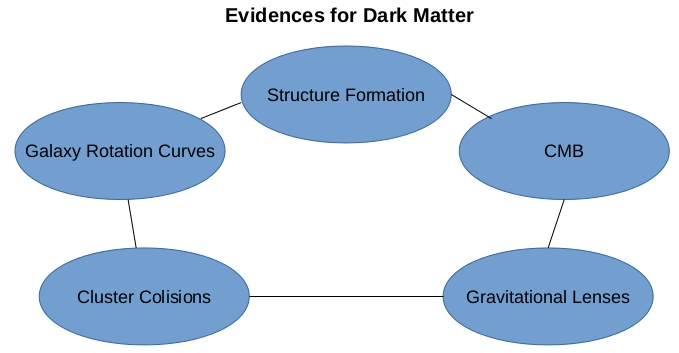
\includegraphics[scale=0.6]{evidences}
\label{fig:evidences}
\caption{Collections of the five most important evidences for Dark Matter. Hacer gáfica...}
\end{figure}

Decribe each one....

\section{Indirect Detection}



Dark matter particles that populate our universe in galactic and extragalactic scales may self-annihilate and produce a flux of gamma-rays, cosmic-rays, neutrinos, anti-matter which can appear as an excess over the expected background. The flux originated from dark matter annihilation should be proportional to the number density squared of particles, i.e. $\rho_{\chi}^2/m_{\chi}^2$, to the annihilation cross section $\sigma v$, to the element of volume of the sky observed accounted by $\Omega$, and the number of particles of interest produced per annihilation ($dN/dE$). Hence, it can we written as,

\begin{equation}
\underbrace{\frac{d\Phi}{d\Omega dE}}_{Diff. Flux} = {\color{blue} \frac{ \underbrace{ \sigma v }_{Anni.\, Cross\, Section}}{8\pi m_{\chi}^2}} \times {\color{green} \underbrace{\frac{dN}{dE}}_{Energy\, Spectrum}} \times {\color{red} \int_{l.o.s} ds} {\color{red}  \underbrace{\rho^2 (\overrightarrow{r}(s,\Omega))}_{Dark\, Matter\, Distribution}},
\label{eq:flux}
\end{equation}where $\Omega$ is truly the solid angle of the region of interest, $dN/dE$ is the energy spectrum (e.g. the number of photons produced per annihilation in case of gamma-rays), and $\rho (\overrightarrow{r}(s,\Omega))$ is the dark matter density which should integrated over the line of sight (l.o.s) from the observer to the source, which is often assumed to be described by either a Navarro-Frenk-White,
\begin{equation}
\rho(r) \propto \frac{r_s}{r[1+ r/r_s]^2},
\end{equation}or Einasto profile,
\begin{equation}
\rho(r) \propto exp \left[ \frac{-2.0}{\alpha} \left(\,  (r/r_s)^{\alpha}-1 \right) \right],
\end{equation}where $r_s=20$~kpc is the scale radius of the halo, and $\alpha=0.17$.



perfiles...